\documentclass[12pt]{article}

\usepackage{minted}
\usepackage{hyperref}
\usepackage{datetime}
\usepackage{datenumber}
\usepackage{pdfpages}
\usepackage{advdate}
\usepackage[super]{nth}
\usepackage[margin=0.75in]{geometry}

\parindent 0pt \parskip 6pt


\begin{document}

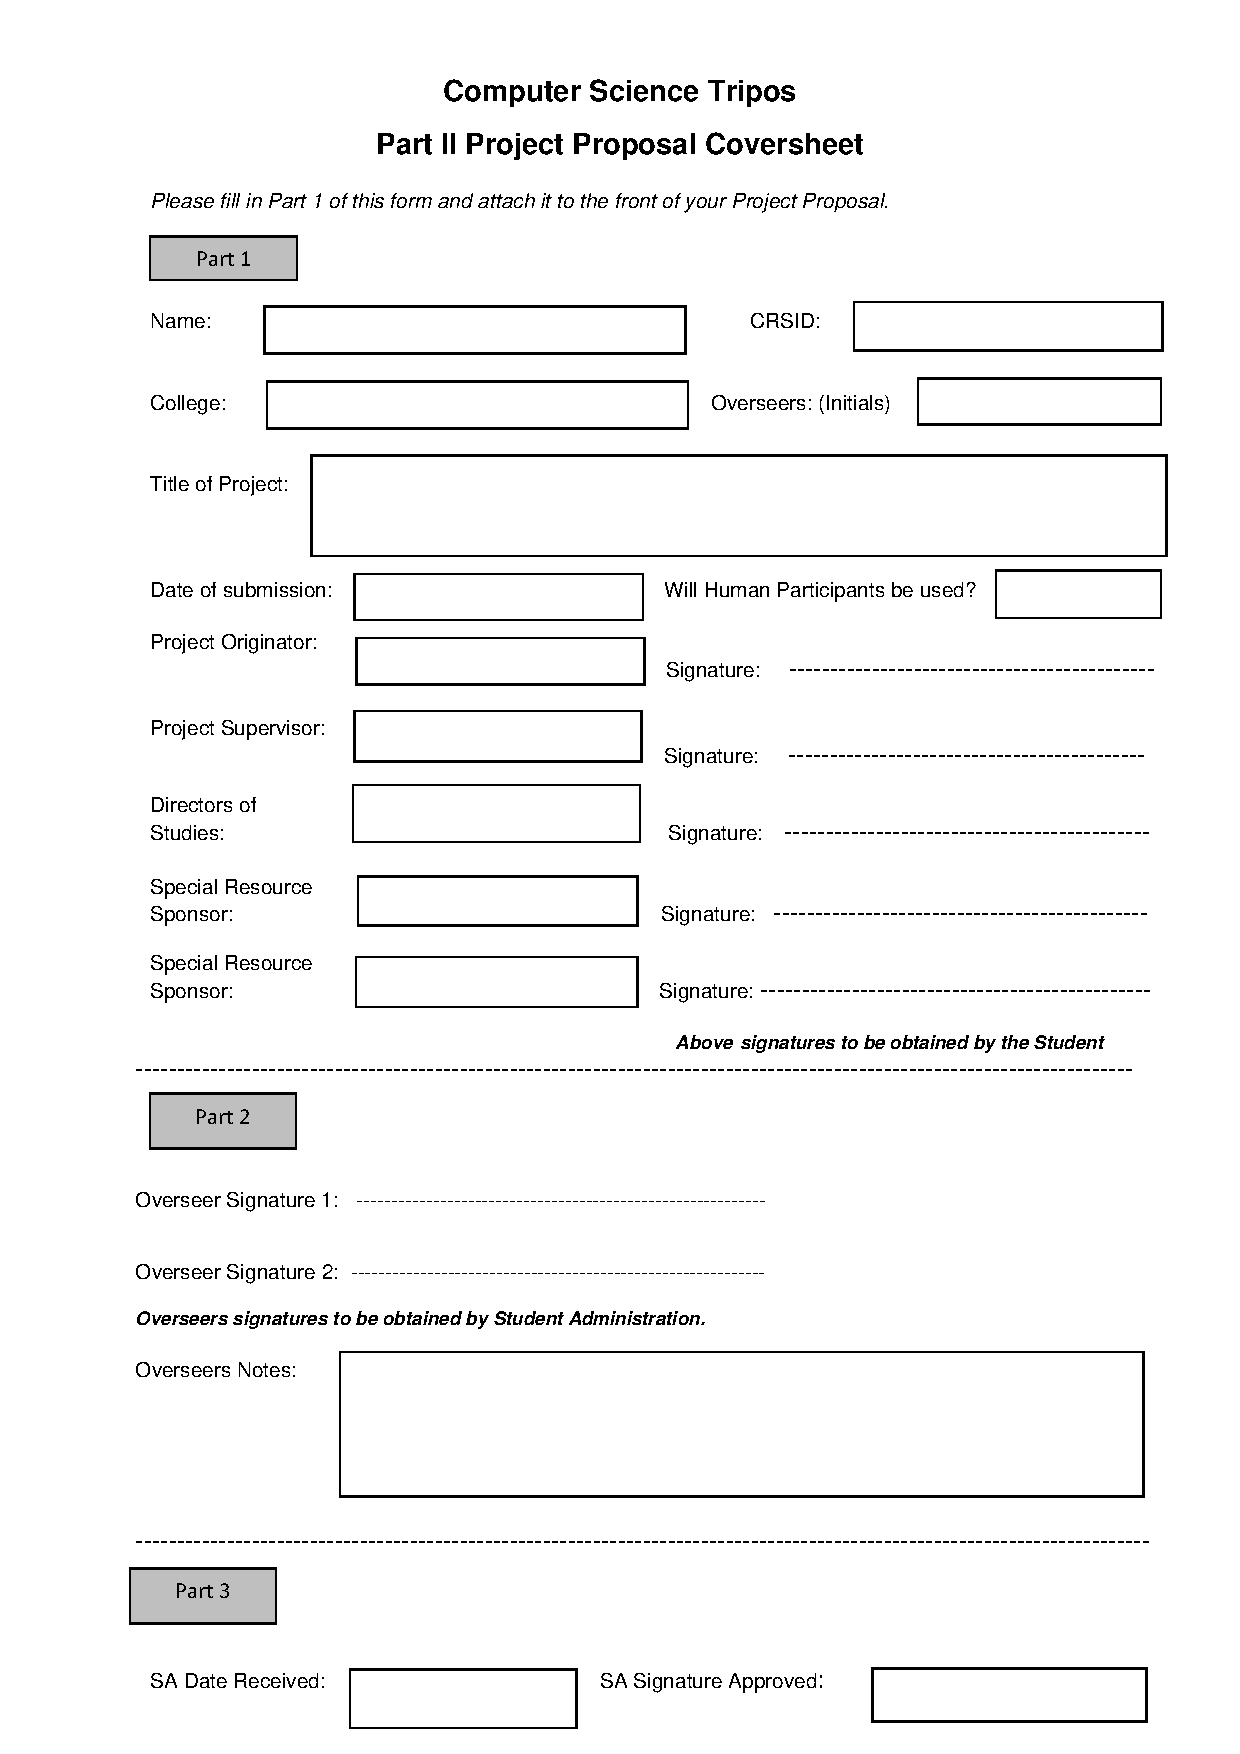
\includepdf[pages={1}]{ProposalForm.pdf}

\thispagestyle{empty}

\centerline{\large Computer Science Tripos: Part II Project Proposal}
\vspace{0.4in}
\centerline{\Large\bf Measuring mutual information within Neural networks}
\vspace{0.3in}

\centerline{Andrius Grabauskas, ag939}
\centerline{Robinson College}

\centerline{\large \textbf{\today}}

\vspace{1in}

\begin{tabular}{ p{4cm} p{4.5cm} l }
{\bf Project Originator:} & Andrius Grabauskas & \\[3mm]
{\bf Project Supervisor:} & Dr.\ Damon Wischik \\[3mm]
{\bf Director of Studies:} & Prof.\ Alan Mycroft \\[3mm]
{\bf Overseers:} & Dr.\ Robert Mullins & Prof.\ Pietro Lio' \\[3mm]
\end{tabular}

\vspace{0.75in}

\section*{Introduction and Description of the Work}

The goal of this project is to confirm or deny the results produced by
Shwartz-ziv \& Tishby in their paper ``Opening the black box of Deep Neural
Networks via Information``\footnote{https://arxiv.org/abs/1703.00810}

The paper tackles our understating of Deep Neural Networks (DNNs). As of yet
there is no comprehensive theoretical understanding of how DNNs learn from data.
The authors proposed to measure how information travels within the DNNs layers.

They found that training of neural networks can be split into to two distinct
phases: memorization followed by the compression phase.
\begin{itemize}
  \item memorization - each layer increases information about the input and the
    label
  \item compression  - this is the generalization stage where each layer tries
    to forget details about the input while still increasing mutual information
    with the label thus improving performance of the DNN. This phase takes the
    wast majority of the training time.
\end{itemize}

They found that each layer in neural network tries to throw out unnecessary data
from the input while preserving information about the output/label. As the
network is trained each layer preserves more information about the label

The results they found were interesting but also contentious as they have not
yet provided a formal proof, just experimental data as a result there are many
peers that are cautious and sceptical of the theory even a
paper\footnote{https://openreview.net/pdf?id=ry\_WPG-A-} was produced that tries
to suggest that the theory is wrong, however this was dismissed by Tishby \&
Shwartz-Ziv\footnote{https://openreview.net/forum?id=ry\_WPG-A-\&noteId=S1lBxcE1z}


\section*{Starting Point}

I have watched a talk that Prof.\ Tishby gave on this topic at Yandex, no other
preparation was done. 

\section*{Resources Required}

I will use my own laptop to train and evaluate the neural networks as I expect
them to be small given the difficulty of measuring mutual information and
entropy in neural networks.

For backups I intend to store my work on GitHub and my own personal machine. In
case my laptop breaks I will get another one or use the MCS machines.

\section*{Substance and Structure of the Project}

The aim of this project to reproduce the results provided by Prof.\ Tishby and
his colleagues. The intention of my work is to help settle the debate surrounding the
topic either strengthening the arguments in favour of the theory in case my
results are inline with the aforementioned results or encourage discussion in
case my results contradict the theory.

My work will require me to have a comprehensive understanding of Information
theory, Information bottleneck and neural networks.

One of the more contentious parts of my project will be measuring mutual
information between the input a layer in the DNN and the label. Mutual
information is known to be tricky to measure when it comes to continuous random
variables.

Will need to use Python to train the neural networks and GNUplot or alternative
to plot the results.

%TODO(ag939) confirm with @damon.wischik in which cases is mutual information is
%tricky to measure ? And also is it computationally expensive to do so?

%TODO(ag939) confirm with @damon.wischik how much compute resources my project
%will require.

\section*{Success Criteria}

Confirm or deny the results produced in``Opening the black box of Deep Neural
Networks via Information`` paper on the same dataset as the paper. In order to do
that I will need to:

\begin{itemize}
    %TODO(ag939) clarify what dataset was used in the paper.
  \item Train a neural network on the same dataset that is used in the paper. I
    will need to train the DNN multiple times in order to make sure the results
    hold irrespective of the neuron weights. I expect a single training round to
    be quite light on the computational resources required but since I will need
    to retrain it multiple times I might need to use compute provided by the
    Computer Lab.
  \item Measure the mutual information between input the layers and the label. I
    will need to measure how information travels between layers this might be
    tricky because as I understand measuring information is know to be difficult
    to get right.
  \item And lastly I will need to analyze the results, compare them to the
    papers finding and address any discrepancies found.
\end{itemize}

\section*{Extensions}

% TODO(ag939) ask @damon.wischik if he has any datasets in mind so that I can
% note them here ?
Provided I achieve the success criteria I am planning to explore other datasets
and try to verify that the theory holds.
% TODO(ag939) clarify what dataset was used in the Paper.
The dataset used in the original paper is very non-standard so it would be very
interesting to see how the theory holds up when we use it with different
datasets.

% TODO(ag939) clarify this with @damo.wishcik.
Different datasets will most likely need different ways to approximate mutual
information between layers.

\section*{Schedule}

% Set start date to 15th October 2018
\ThisYear{2018}\ThisMonth{10}\ThisDay{15}

% Specify date format like "15th Oct"
\newdateformat{datefmt}{\nth{\THEDAY} \shortmonthname[\THEMONTH]}

% Force advdate commands to change the global "today" instance, not the local one
\makeatletter
\renewcommand\AdvanceDate[1][\@ne]{\global\advance\day#1 \FixDate}
\renewcommand\FixDate{%
  \FixMonth \is@LeapYear
  \l@@p \global\ifnum\day<1 \Pr@vD@y \repeat
  \l@@p \M@s\m@sic \global\ifnum\day>\M@s \N@xtD@y \repeat
}
\renewcommand\FixMonth{%
  \L@@p \global\ifnum\month<1 \global\advance\year\m@ne \global\advance\month12 \is@LeapYear \repeat
  \L@@p \global\ifnum\month>12 \global\advance\year\@ne \global\advance\month-12 \is@LeapYear \repeat}
\def\Pr@vD@y{%
  \global\ifnum\day<-366
    \global\ifnum\month>2
      \global\advance\day\r@k \global\advance\year\m@ne \is@LeapYear
    \else
      \global\advance\year\m@ne \is@LeapYear \advance\day\r@k
    \fi
  \else
    \global\advance\month\m@ne \FixMonth
    \global\advance\day\m@sic
  \fi}
\def\N@xtD@y{%
  \global\ifnum\day>366
    \global\ifnum\month>2
      \global\advance\year\@ne \is@LeapYear \global\advance\day-\r@k
    \else
      \global\advance\day-\r@k \global\advance\year\@ne \is@LeapYear
    \fi
  \else
    \global\advance\day-\M@s \global\advance\month\@ne \FixMonth
  \fi}
\makeatother

% Output eg. boldface "15th Oct - 29th Oct" when called.
\newcommand{\daterange}[1]{%
    \textbf{\datefmt\today}
    \textbf{--}
    \AdvanceDate[#1]\relax
    \AdvanceDate[-1]\relax
    \textbf{\datefmt\today}
    \AdvanceDate[1]\relax
}

\begin{itemize}
  \item {
      \daterange{21}

      At the start of my dissertation I expect to spend quite a bit of time
      reading up on the relevant subjects
      \begin{itemize}
        \item { 
          Information theory primarily will read Mackay`s
          book\footnote{Informaition Theory, Inference, and Learning Algorithms
          by David J. C. MacKay} 
        } \item { 
          Information bottleneck will use relevant papers and talks.
        } \item {
          Training neural networks. 
        } \item {
          Measuring Entropy and Mutual information between DNN layers
        }
      \end{itemize}
  } \item {
      \daterange{14}

      At this point I should be confident enough with the theory proposed by
      Tishby and will start examining the code that was
      provided\footnote{https://github.com/ravidziv/IDNNs}.  I will need to
      learn the relevant technologies for training neural networks.
  } \item {
      \daterange{14}

      Having examined Tishby`s code I will reimplement it both in order to
      understand it better and for the cause of independent verification.
  } \item {
      \daterange{35}

      Having a working system to test data sets I will try to reproduce results
      from the paper on the same dataset. This will achieve my success criteria.
  } \item {
      \daterange{42}

      Assuming everything goes as planned I will start looking into other
      datasets to verify the theory still stands and is not just a consequence
      of the dataset chosen in the paper.
  } \item {
      \daterange{28}

      Will use the remaining time to write up the dissertation.
  }
\end{itemize}

\end{document}
